\documentclass{standalone}
\usepackage{tikz}
\begin{document}
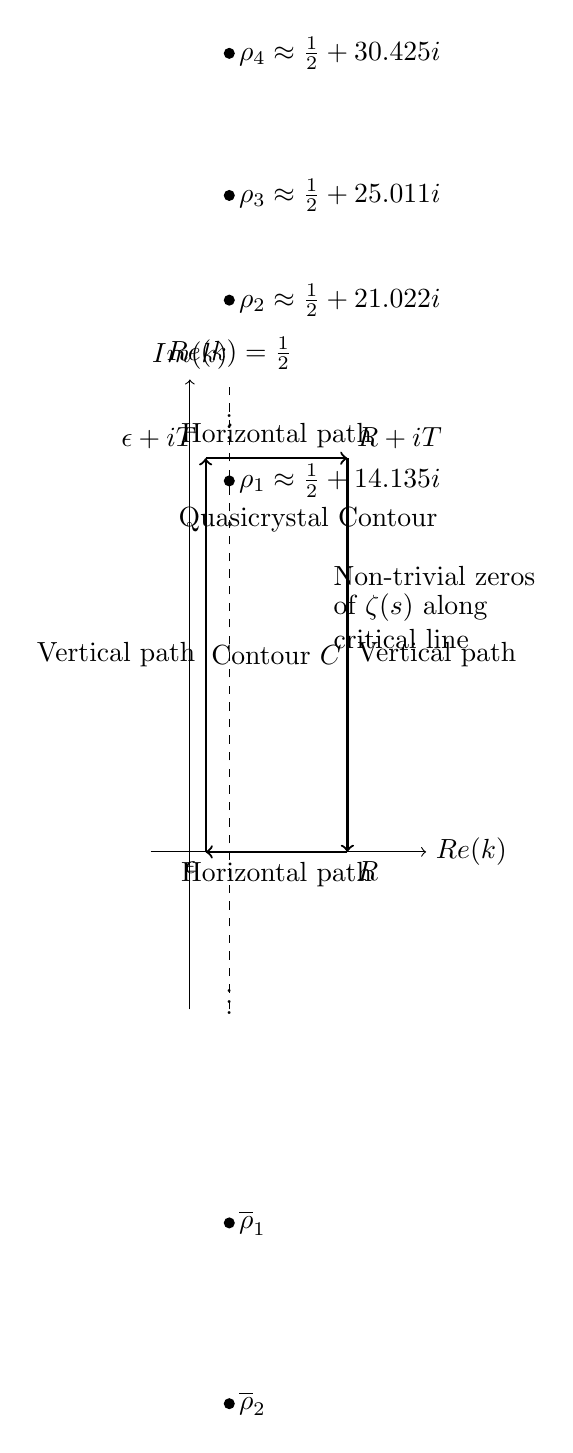
\begin{tikzpicture}
% Axes
\draw[->] (-0.5,0) -- (3,0) node[right] {$\text{Re}(k)$};
\draw[->] (0,-2) -- (0,6) node[above] {$\text{Im}(k)$};

% Critical line
\draw[dashed] (0.5,-2) -- (0.5,6) node[above] {$\text{Re}(k) = \frac{1}{2}$};

% Contour path (counterclockwise)
\draw[thick,->] (2,0) -- (0.2,0) node[midway,below] {Horizontal path};
\draw[thick,->] (0.2,0) -- (0.2,5) node[midway,left] {Vertical path};
\draw[thick,->] (0.2,5) -- (2,5) node[midway,above] {Horizontal path};
\draw[thick,->] (2,5) -- (2,0) node[midway,right] {Vertical path};

% Non-trivial zeros (poles) of the Riemann zeta function
\fill (0.5,14.135/3) circle (2pt) node[right] {$\rho_1 \approx \frac{1}{2} + 14.135i$};
\fill (0.5,21.022/3) circle (2pt) node[right] {$\rho_2 \approx \frac{1}{2} + 21.022i$};
\fill (0.5,25.011/3) circle (2pt) node[right] {$\rho_3 \approx \frac{1}{2} + 25.011i$};
\fill (0.5,30.425/3) circle (2pt) node[right] {$\rho_4 \approx \frac{1}{2} + 30.425i$};

% Indicate more zeros
\node at (0.5,5.5) {$\vdots$};

% Also show reflection symmetry
\fill (0.5,-14.135/3) circle (2pt) node[right] {$\overline{\rho}_1$};
\fill (0.5,-21.022/3) circle (2pt) node[right] {$\overline{\rho}_2$};
\node at (0.5,-1.8) {$\vdots$};

% Labels for vertices
\node[below left] at (0.2,0) {$\epsilon$};
\node[above left] at (0.2,5) {$\epsilon + iT$};
\node[above right] at (2,5) {$R + iT$};
\node[below right] at (2,0) {$R$};

% Annotation for contour
\node at (1.1,2.5) {Contour $C$};
\node[below] at (1.5,4.5) {Quasicrystal Contour};
\node[right] at (1.7,3.5) {Non-trivial zeros};
\node[right] at (1.7,3.1) {of $\zeta(s)$ along};
\node[right] at (1.7,2.7) {critical line};
\end{tikzpicture}
\end{document}
